\fancyhead[C]{Section 15.3}
	\fancyhead[R]{\dayfifteen}
\iftoggle{questions}{
\begin{center}{\large \textbf{Math 2551 Worksheet: Applications of Double Integrals}}
\end{center}

\begin{enumerate}
	
	\item The figure below shows a temperature map of Colorado. Use the data to estimate the average temperature in the state using 4, 16, and 25 subdivisions.  Give both an upper and lower estimate for each number of subdivisions.  Why do we like Colorado for this problem?  What other state(s) or countries might we like?
	\begin{center}
		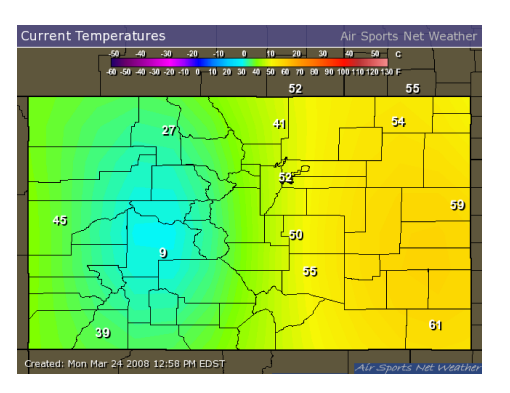
\includegraphics[scale=0.9]{colorado_temp.png}
	\end{center}
	
	\item Which do you think will be larger, the average value of $f(x,y)=xy$ over the square $0\leq x \leq 1, 0\leq y\leq 1$, or the average value of $f$ over the quarter circle $x^2+y^2\leq 1$ in the first quadrant? Calculate them to find out. 
	
	\item If $f(x,y)=100(y+1)$ represents the population density in people per square mile of a planar region on Earth, where $x$ and $y$ are measured in miles, find the number of people in the region bounded by the curves $x=y^2$ and $x=2y-y^2$.
	
\end{enumerate}
}{}

\iftoggle{answers}{
\begin{center}{\large \textbf{Math 2551 Worksheet 16 Answers: Applications, Polar Double Integrals}}
\end{center}

\begin{enumerate}
	\item Answers will vary a bit through the estimation process
	
	4 subdivisions: $31.75 \leq T_{avg} \leq 52.5$\\
	16 subdivisions: $33.18  \leq T_{avg} \leq 50.06$\\
	25 subdivisions: $36.32  \leq T_{avg} \leq 49.8$\\
	
	Colorado is a rectangle, which makes it easy to subdivide. Wyoming would also work well.
	
	
	\item On square: $f_{avg}=\frac{1}{1}\cdot \frac{1}{4}=\frac{1}{4}$\\
	
	On quarter circle: $f_{avg}=\frac{1}{\pi/4}\cdot \frac{1}{8}=\frac{1}{2\pi}$ 
	\item 50 people
\end{enumerate}
}{}
\iftoggle{solutions}
{
Solutions go here in the same format.
}{}